\documentclass[12pt]{article}
%\usepackage{scicite}
\usepackage{times}
\usepackage{hyperref}
\usepackage{setspace}
\usepackage{amsmath}
\usepackage{listings}
\usepackage{graphicx}


\makeatletter
\renewcommand*\env@matrix[1][*\c@MaxMatrixCols c]{%
  \hskip -\arraycolsep
  \let\@ifnextchar\new@ifnextchar
  \array{#1}}
\makeatother

\topmargin 0.0cm
\oddsidemargin 0.2cm
\textwidth 16cm 
\textheight 21cm
\footskip 1.0cm

%The next command sets up an environment for the abstract to your paper.

\newenvironment{sciabstract}{%
\begin{quote} \bf}
{\end{quote}}


% If your reference list includes text notes as well as references,
% include the following line; otherwise, comment it out.

%\renewcommand\refname{References}

% The following lines set up an environment for the last note in the
% reference list, which commonly includes acknowledgments of funding,
% help, etc.  It's intended for users of BibTeX or the {thebibliography}
% environment.  Users who are hand-coding their references at the end
% using a list environment such as {enumerate} can simply add another
% item at the end, and it will be numbered automatically.




% Include your paper's title here

\title{FYS4150 Project 1} 
\author
{Mikkel Killingmoe Christensen\\
\\
\normalsize{\today}
}

% Include the date command, but leave its argument blank.

\date{}
%%%%%%%%%%%%%%%%% END OF PREAMBLE %%%%%%%%%%%%%%%%



\begin{document} 

% Double-space the manuscript.

\baselineskip24pt

% Make the title.

\maketitle 



% Place your abstract within the special {sciabstract} environment.
\begin{center}
\par GitHub repository:
\par \url{https://github.com/mikkello/FYS4150/}
\end{center}
\begin{center}
{\large \textbf{Abstract}}
\end{center}
\begin{sciabstract}
A reliable and fast method for solving second degree differential equations numerically is needed as these problems often occur in physics and other sciences. In this project, a second degree differential equation was converted to a matrix equation to be solved numerically by Gaussian elimination and LU decomposition algorithms. The different algorithms was compared in terms of speed and relative error. It was found that a modified Gaussian elimination algorithm was the fastest, and that LU decomposition required to much computation time to be used for large matrices and small step sizes. It was also found that small step sizes can lead to loss of numerical precision.   
\end{sciabstract}



\section{Introduction}
In this project, the goal was to find a numerical solution to a second degree differential equation. An example of such an equation is Poisson's equation in electromagnetism given by:
\begin{equation}
\frac{d^{2} \phi}{dr^{2}}=-4 \pi r\rho (r)
\end{equation}

This type of differential equation can be rewritten as the following with Dirichlet boundary conditions:
\begin{equation}
-u^{''}(x)=f(x), \quad x\in(0,1), \quad u(0)=u(1)=0
\end{equation}



\section{Theory}
\subsection{Poisson equation}
To solve the one-dimensional Poisson equation with Dirchelet boundary conditions, an approximation of the second derivative is made using Taylor expansion:
\begin{equation}
\frac{d^{2}u}{dx^{2}}\approx\frac{u(x+h)+u(x-h)-2u(x)}{h^{2}}+O(h^{2})
\end{equation}
where $O(h^{2})$ is the truncation error. 

The equation is then discretized and a simpler notation is used to yield the following:

\begin{equation}
\frac{u_{i+1}+u_{i-1}-2u_{i}}{h^{2}}=-f_{i}
\end{equation}

The step size is given by:
\begin{equation}
h = \frac{1}{n+1}
\end{equation}

Furthermore, the equation is a system of linear equations and can thus be written as a linear equation using linear algebra. The equation reads as follows:
\begin{equation}
\mathbf{A}u=h^{2}\mathbf{f}
\end{equation}
with
\begin{equation}
\mathbf{A} = \begin{bmatrix}
                           2& -1& 0 &\dots   & \dots &0 \\
                           -1 & 2 & -1 &0 &\dots &\dots \\
                           0&-1 &2 & -1 & 0 & \dots \\
                           & \dots   & \dots &\dots   &\dots & \dots \\
                           0&\dots   &  &-1 &2& -1 \\
                           0&\dots    &  & 0  &-1 & 2 \\
                      \end{bmatrix}
                      \label{eq:tridiagm}
\end{equation}
being a tridiagonal  $n\times n$ matrix. The problem is now possible to solve by finding the vector $\mathbf{u}$. For small matrices, this can easily be done by multiplying both sides with the inverse of $\mathbf{A}$. For larger matrices, however, this procedure is slow and a better method is needed. 

\subsubsection{Analytical solution}
Analytical solutions exists for the Poisson equation problem, and it will be useful to compare this to the numerical results. 
For the term:
\begin{equation}
f(x) = 100e^{-10x}
\end{equation}
the exact solution is:
\begin{equation}
u(x) = 1-(1-e^{-10})x-e^{-10x}
\end{equation}

\subsection{Guassian elimination}
Guassian elimination is an efficient method for solving these types of equations. The matrix is here transformed into the identity matrix, while a new vector $\tilde{d}$ is created with the solution. 

The elimination is here shown with a generalized 4x4 matrix, but the method works for any $n\times n$ matrix. 

\begin{equation}
\begin{bmatrix}
                           a_{1}&b_{1}&0&0 \\
                           c_{1}&a_{2}&b_{2}&0\\
                           0&c_{2}&a_{3}&b_{3}\\
                           0&0&c_{3}&a_{4}
                      \end{bmatrix}
                      \begin{bmatrix}
                           u_{1} \\
                           u_{2}\\
                           u_{3}\\
                           u_{4}
                      \end{bmatrix}
                      =
                      \begin{bmatrix}
                           d_{1} \\
                           d_{2}\\
                           d_{3}\\
                           d_{4}
                      \end{bmatrix}
\end{equation}
\subsubsection{Forward substitution}
To remove the elements below the diagonal in the matrix, the method of forward substitution is used. The first operation is to subtract $\frac{c_{1}}{a_{1}}$ times the first row. 
This will create an extended matrix looking like this: 
\begin{equation}
\begin{bmatrix}[cccc|c]
                           a_{1}&b_{1}&0&0& d_{1}\\
                           c_{1}&a_{2}&b_{2}&0& d_{2}\\
                           0&c_{2}&a_{3}&b_{3}& d_{3}\\
                           0&0&c_{3}&a_{4}& d_{4}
                      \end{bmatrix}
                      \sim
                      \begin{bmatrix}[cccc|c]
                           a_{1}&b_{1}&0&0& d_{1}\\
                           0&a_{2}-\frac{c_{1}b_{1}}{a_{1}}&b_{2}&0& d_{2}-\frac{d_{1}c_{1}}{a_{1}}\\
                           0&c_{2}&a_{3}&b_{3}& d_{3}\\
                           0&0&c_{3}&a_{4}& d_{4}
\end{bmatrix}
\end{equation}
These operations can be generalized by introducing the new variables
\begin{equation}
\tilde{a}_{i}=a_{i}-\frac{b_{i-1}c_{i-1}}{\tilde{a}_{i-1}}
\end{equation}
\begin{equation}
\tilde{d}_{i}=d_{i}-\frac{\tilde{d}_{i-1}c_{i-1}}{\tilde{a}_{i-1}}
\end{equation}
Continuing the row reduction with the forward substitution starting with the lowest index of the c-diagonal will yield the following equation:

\begin{equation}
\begin{bmatrix}
                           \tilde{a}_{1}&b_{1}&0&0\\
                           0&\tilde{a}_{2}&b_{2}&0\\
                           0&0&\tilde{a}_{3}&b_{3}\\
                           0&0&0&\tilde{a}_{4}
                      \end{bmatrix}
                      \begin{bmatrix}
                           u_{1} \\
                           u_{2}\\
                           u_{3}\\
                           u_{4}
                      \end{bmatrix}
                      =
                      \begin{bmatrix}
                           \tilde{d}_{1} \\
                           \tilde{d}_{2}\\
                           \tilde{d}_{3}\\
                           \tilde{d}_{4}
                      \end{bmatrix}
\end{equation}
with the boundary conditions $\tilde{a}_{1}=a_{1}$ and $\tilde{d}_{1}=d_{1}$

The two formulas in the forwards substitution requires three floating point operations each, yielding a total of $6(n-1)$ FLOPS.
\subsubsection{Backward substitution}
To remove the elements above the diagonal in the matrix, the method of backward substitution is used. As opposed to the forward substitution, we start with the highest index of the b-diagonal. The first operation is to remove $b_{3}$ by subtracting the third row with $\frac{b_{3}}{\tilde{a}_{4}}$ times the fourth row. 

\begin{equation}
\begin{bmatrix}[cccc|c]
                           \tilde{a}_{1}&b_{1}&0&0&\tilde{d}_{1}\\
                           0&\tilde{a}_{2}&b_{2}&0&\tilde{d}_{2}\\
                           0&0&\tilde{a}_{3}&b_{3}&\tilde{d}_{3}\\
                           0&0&0&\tilde{a}_{4}&\tilde{d}_{4}
                      \end{bmatrix}
                      \sim
                      \begin{bmatrix}[cccc|c]
                           \tilde{a}_{1}&b_{1}&0&0& \tilde{d}_{1}\\
                           0&\tilde{a}_{2}&b_{2}&0& \tilde{d}_{2}\\
                           0&0&\tilde{a}_{3}&0& \tilde{d}_{3}-\frac{b_{3}\tilde{d}_{4}}{\tilde{a}_{4}}\\
                           0&0&0&\tilde{a}_{4}& \tilde{d}_{4}
                      \end{bmatrix}
\end{equation}
Repeating the procedure on the other rows will remove $b_{2}$ and $b_{3}$ and yield the following matrix:
\begin{equation}
\begin{bmatrix}[cccc|c]
\tilde{a}_{1}&0&0&0&\tilde{d}_{1}-\frac{b_{1}}{\tilde{a}_{3}}(\tilde{d}_{2}-\frac{b_{2}}{\tilde{a}_{3}}(\tilde{d}_{3}-\frac{b_{3}\tilde{d}_{4}}{\tilde{a}_{4}})) \\
0&\tilde{a}_{2}&0&0&\tilde{d}_{2}-\frac{b_{2}}{\tilde{a}_{3}}(\tilde{d}_{3}-\frac{b_{3}\tilde{d}_{4}}{\tilde{a}_{4}})\\
0&0&\tilde{a}_{3}&0&\tilde{d}_{3}-\frac{b_{3}\tilde{d}_{4}}{\tilde{a}_{4}}\\
0&0&0&\tilde{a}_{4}&\tilde{d}_{4}

\end{bmatrix}
\end{equation}
Putting this new matrix into the linear equation, the following relations can be found:
\begin{equation}
u_{4}=\frac{\tilde{d}_{4}}{\tilde{a}_{4}}
\end{equation}
and
\begin{equation}
u_{3}=\frac{\tilde{d}_{3}-b_{3}u_{4}}{\tilde{a}_{3}}
\end{equation}
Generalizing this to a matrix with i-rows, the following formula for $u_{i}$ can be found:
\begin{equation}
u_{i}=\frac{\tilde{d}_{i}-b_{i}u_{i+1}}{\tilde{a}_{i}}
\end{equation}
This formula requires three floating point operations, yielding a total of $3(n-1)$ FLOPS. This means that the full Guassian elimination requires $9(n-1)$ FLOPS. 


\subsubsection{Numerical implementation of the Gaussian elimination}
This is a code snippet showing how the Gaussian elimination can be implemented in Python. 
\lstset{language=Python}
\lstset{frame=lines}
\lstset{caption={Implementing the Gaussian elimination algorithms in Python}}
\lstset{label={lst:code_direct}}
\lstset{basicstyle=\footnotesize}
\begin{lstlisting}
# Forward substitution
	for i in range(n-1):  
		a_t[i+1] -= (b[i]*c[i]) / a_t[i]
		d[i+1] -= (b[i]*d[i]) / a_t[i]
# Backwards substitution
	for i in range(n-1,1,-1): 
		d[i-1] -= (c[i-1]*d[i]) / a_t[i]
\end{lstlisting}

\subsubsection{Gaussian elimination of a tridiagonal matrix}
The matrix (\ref{eq:tridiagm}) used in this problem is a tridiagonal matrix with two of the diagonals being $-1$, also calles a Toeplitz matrix. This will simplify the algorithms and save FLOPS.

Updating the Guassian elimination formulas with this special case, yields the following new equations:

\begin{equation}
\tilde{a}_{i}=\tilde{a}_{i}+\frac{b_{i-1}}{\tilde{a}_{i-1}}
\end{equation}
which can be further simplified to:
\begin{equation}
\tilde{a}_{i}=\frac{i+1}{i}
\label{eq:a_i}
\end{equation}
\begin{equation}
\tilde{d}_{i}=d_{i}+\frac{\tilde{d}_{i-1}}{\tilde{a}_{i-1}}
\end{equation}
\begin{equation}
u_{i}=\frac{\tilde{d}_{i}+u_{i+1}}{\tilde{a}_{i}}
\end{equation}

The new set of equations will require $4(n-1)$ FLOPS, which is a great reduction in the required computation power. Equation (\ref{eq:a_i}) can be pre-calculated outside the algorithm and will therefore not add more FLOPS.

\subsubsection{Numerical implementation of the special case}
This is a code snippet showing how the Gaussian elimination for the special case can be implemented in Python. 
\lstset{language=Python}
\lstset{frame=lines}
\lstset{caption={Implementing the Gaussian elimination algorithms in Python for the special case}}
\lstset{label={lst:code_direct2}}
\lstset{basicstyle=\footnotesize}
\begin{lstlisting}
for i in range(1,n,1):
		d_t[i] = d[i] + d_t[i-1] / a_t[i-1]
        

for i in range(n-2, 0, -1):
		u[i] = (d_t[i]+u[i+1]) / a_t[i]
return u
\end{lstlisting}

\subsection{LU-decomposition}
Decomposing a matrix in one lower triagonal and one upper triagonal matrix is called LU-decomposition. This can be done to split a matrix equation into to new equations which makes the problem easier to solve. 
The matrix equation $A\mathbf{u}=\mathbf{v}$ will then read:
\begin{equation}
LU\mathbf{u}=\mathbf{v}
\end{equation}
After introducing $\mathbf{y}=U\mathbf{u}$, the solution can be computed. First $\mathbf{y}$ is found from:
\begin{equation}
L\mathbf{y}=\mathbf{v}
\end{equation}
Then, \begin{equation}
U\mathbf{u}=y
\end{equation}
can be solved to find $\mathbf{u}$. 
	The drawback of using LU decomposition to solve matrix equations numerically, is the fact that the algorithm requires $n^{3}$ FLOPS, which is $n^{2}$ times more than for Guassian elimination. 
\section{Method and results}
\subsection{Plot of the analytical solution}
The analytical solution was plotted to get a feeling of what the numerical solution would look like. It can be seen in figure (\ref{fig:analytical}).

\begin{figure}
\caption{Analytical solution}
\label{fig:analytical}
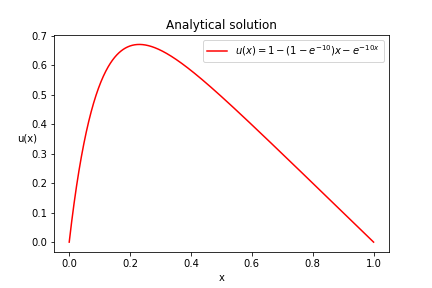
\includegraphics[]{analytical.png}
\end{figure}

\subsection{Implementation of general and special solver}
A Python-program for the two solvers were made (1\textunderscore b.py and 1\textunderscore c.py), and the second derivative for $f(x)=100e^{-10x}$ was calculated and compared with the analytical results for $n = 10^{1}, 10^{2}, ..., 10^{6}$. The computation time and maximum error for the different step sizes and algorithms were also calculated, and these can be found in table (\ref{tab:seconds}) and table (\ref{tab:error})
	The solution from the general algorithm was plotted as a function of x for n = 10 and n = 1000 and compared to the analytical solution. The plots can be seen in figure (\ref{fig:10}) and figure (\ref{fig:1000}). 

\begin{table}[]
\centering
\caption{Computation time for the different algorithms and grid points.}
\label{tab:seconds}
\begin{tabular}{|l|l|l|l|}
\hline
n    & General [s]& Special [s]& LU [s]  \\ \hline
$10^{1}$   & 0.000033        & 0.000029        &  0.000181    \\ \hline
$10^{2}$  & 0.000382        &  0.000210       &  0.000419    \\ \hline
$10^{3}$ & 0.004647       &  0.001499       &  0.033709    \\ \hline
$10^{4}$ & 0.036191       &  0.018247       & 11.567454      \\ \hline
$10^{5}$ & 0.298454       & 0.148838        &  N/A     \\ \hline
$10^{6}$ & 2.787917       & 1.408053        &  N/A    \\ \hline
\end{tabular}
\end{table}

\begin{table}[]
\centering
\caption{The maximum errors for the different algorithms and grid points.}
\label{tab:error}
\begin{tabular}{|l|l|l|}
\hline
n    & General & Special   \\ \hline
$10^{1}$  & 0.616569        & 0.258242              \\ \hline
$10^{2}$  & 0.060437        &  0.015616            \\ \hline
$10^{3}$ & 0.006005        & 0.001955           \\ \hline
\end{tabular}
\end{table}

\begin{figure}
\caption{Comparing the general algorithm to the analytical solution for n=10. The maximum error for this step size is quite large.}
\label{fig:10}
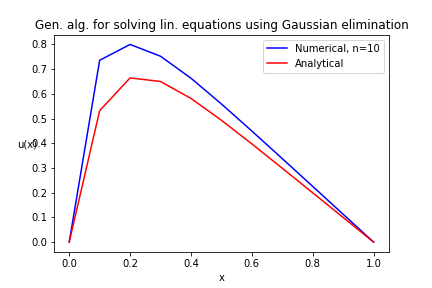
\includegraphics[]{1b_10.png}
\end{figure}

\begin{figure}
\caption{Comparing the general algorithm to the analytical solution for n=1000. The numerical solution is now close to the analytical.}
\label{fig:1000}
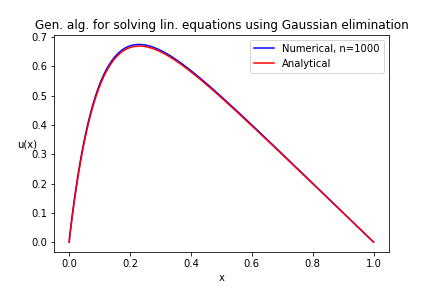
\includegraphics[]{1b_1000.png}
\end{figure}


\subsection{LU decomposition}
The matrix equation was also solved using LU decomposition to compare the computation time for this method to Gaussian elimination. This can also be seen in table (\ref{tab:seconds}).
\subsection{Relative error}
The maximum error as a function of the step size was plotted to see how accurate the approximation from the general Gaussian algorithm were compared to the analytical solution. The plot can be seen in figure (\ref{fig:error}).
\begin{figure}
\caption{The maximum error as a function of step size for the general algorithm. A linear relationship can be seen. }
\label{fig:error}
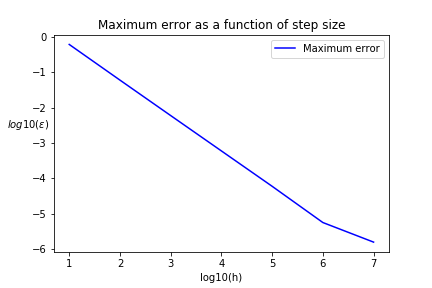
\includegraphics[]{h_epsilon.png}
\end{figure}
\section{Discussion}
\subsection{Computation time}
The special algorithm was expected to be the fastest algorithm because of the lower amount of FLOPS needed to run the algorithm. The general algorithm was expected to be a bit slower, and the LU decomposition was expected to be much slower. It was also expected that the computation time would increase quite linearly with n. This trend was confirmed as seen in table (\ref{tab:seconds}).

\subsection{Errors}
The maximum error was expected do decrease quite fast with increasing n. As seen in figure (\ref{fig:10}), a low n gave a large deviation from the analytical solution. Increasing n to just 1000 (figure (\ref{fig:1000})), gave a much smaller deviation.
	The plot in figure (\ref{fig:error}) shows a linear relationship between the step size and the maximum error, but at $n = 10^{7}$, the linearity is broken. This is most likely due to truncation error because the computer only can store a finite amount of digits. 

\section{Conclusion}
In this project, it was shown that a tridiagonal matrix could be solved by a simple algorithm using Gaussian elimination. It was found that this could save computation time compared to standard LU decomposition. In addition, it was shown that one could get a loss of numerical precision due to small step sizes. 








%-----------------------------------------------------%



\begin{flushleft}

\begin{thebibliography}{}

\singlespacing
\small




  
\bibitem{Article}
  Morten Hjorth-Jensen,
  Computational Physics,
  August 2015
  
\end{thebibliography}
\end{flushleft}






\end{document}




















